\documentclass[12pt, a4paper]{article}

\usepackage[a4paper, margin=2cm]{geometry}
\usepackage{setspace}
\usepackage[portuguese]{babel}
\usepackage{graphicx}
\usepackage{hyperref}
\usepackage{amsfonts}
\usepackage[dvipsnames]{xcolor}

\chardef\_=`_

\title{\textbf{LI3 - Relatório da Fase II - Grupo 12}}
\author{
    Humberto Gomes (A104348) \\
    José Lopes     (A104541) \\
    José Matos     (A100612) \\
}
\date{janeiro de 2024}

\begin{document}
\maketitle
\onehalfspacing
\setlength{\parskip}{\baselineskip}
\setlength{\parindent}{0pt}

\begin{abstract}
    Após a conclusão da primeira fase deste trabalho, procurámos implementar as funcionalidades em
    falta para a conclusão do desenvolvimento desta aplicação: as restantes quatro
    \emph{queries}, um modo de uso interativo (uma interface TUI), testes funcionais e de
    desempenho, e suporte para um \emph{dataset} de maior dimensão, mantendo um desempenho
    aceitável. Adicionalmente, procurámos também melhorar o encapsulamento e a modularidade no
    nosso projeto.
\end{abstract}

\section{Estrutura do trabalho}

Nesta secção, procuramos descrever as diferenças entre a nossa arquitetura modular atual, e a que
tínhamos presente na primeira fase do projeto. Devido ao elevado número de módulos, após o diagrama
de dependências completo que se segue, este documento descreve o funcionamento de cada subsistema
lógico do programa um a um. Nestes esquemas, para reduzir a complexidade visual, não incluímos
todas as relações de dependência, mas apenas as mais relevantes. Segue-se a nossa convenção gráfica:

\begin{itemize}
    \item Um retângulo com cantos arredondados representa uma estrutura de dados;
    \item Um retângulo sem cantos arredondados representa um módulo cuja tarefa principal é a
          execução de código. No entanto, alguns destes módulos podem conter estruturas de dados
          auxiliares (por exemplo, uma gramática definida no módulo de um \emph{parser});
    \item $A \rightarrow B$ significa que o módulo $A$ depende do módulo $B$.
    \item Qualquer módulo ou relação de dependência representado(a) a {\color{ForestGreen}verde}
          indica que o(a) mesmo(a) é uma adição nesta segunda fase, ausente na entrega anterior.
\end{itemize}

% TODO - inserir diagrama global aqui

\subsection{\emph{Parsing}}
\label{sec:parsing}

\begin{figure}[ht]
    \centering
    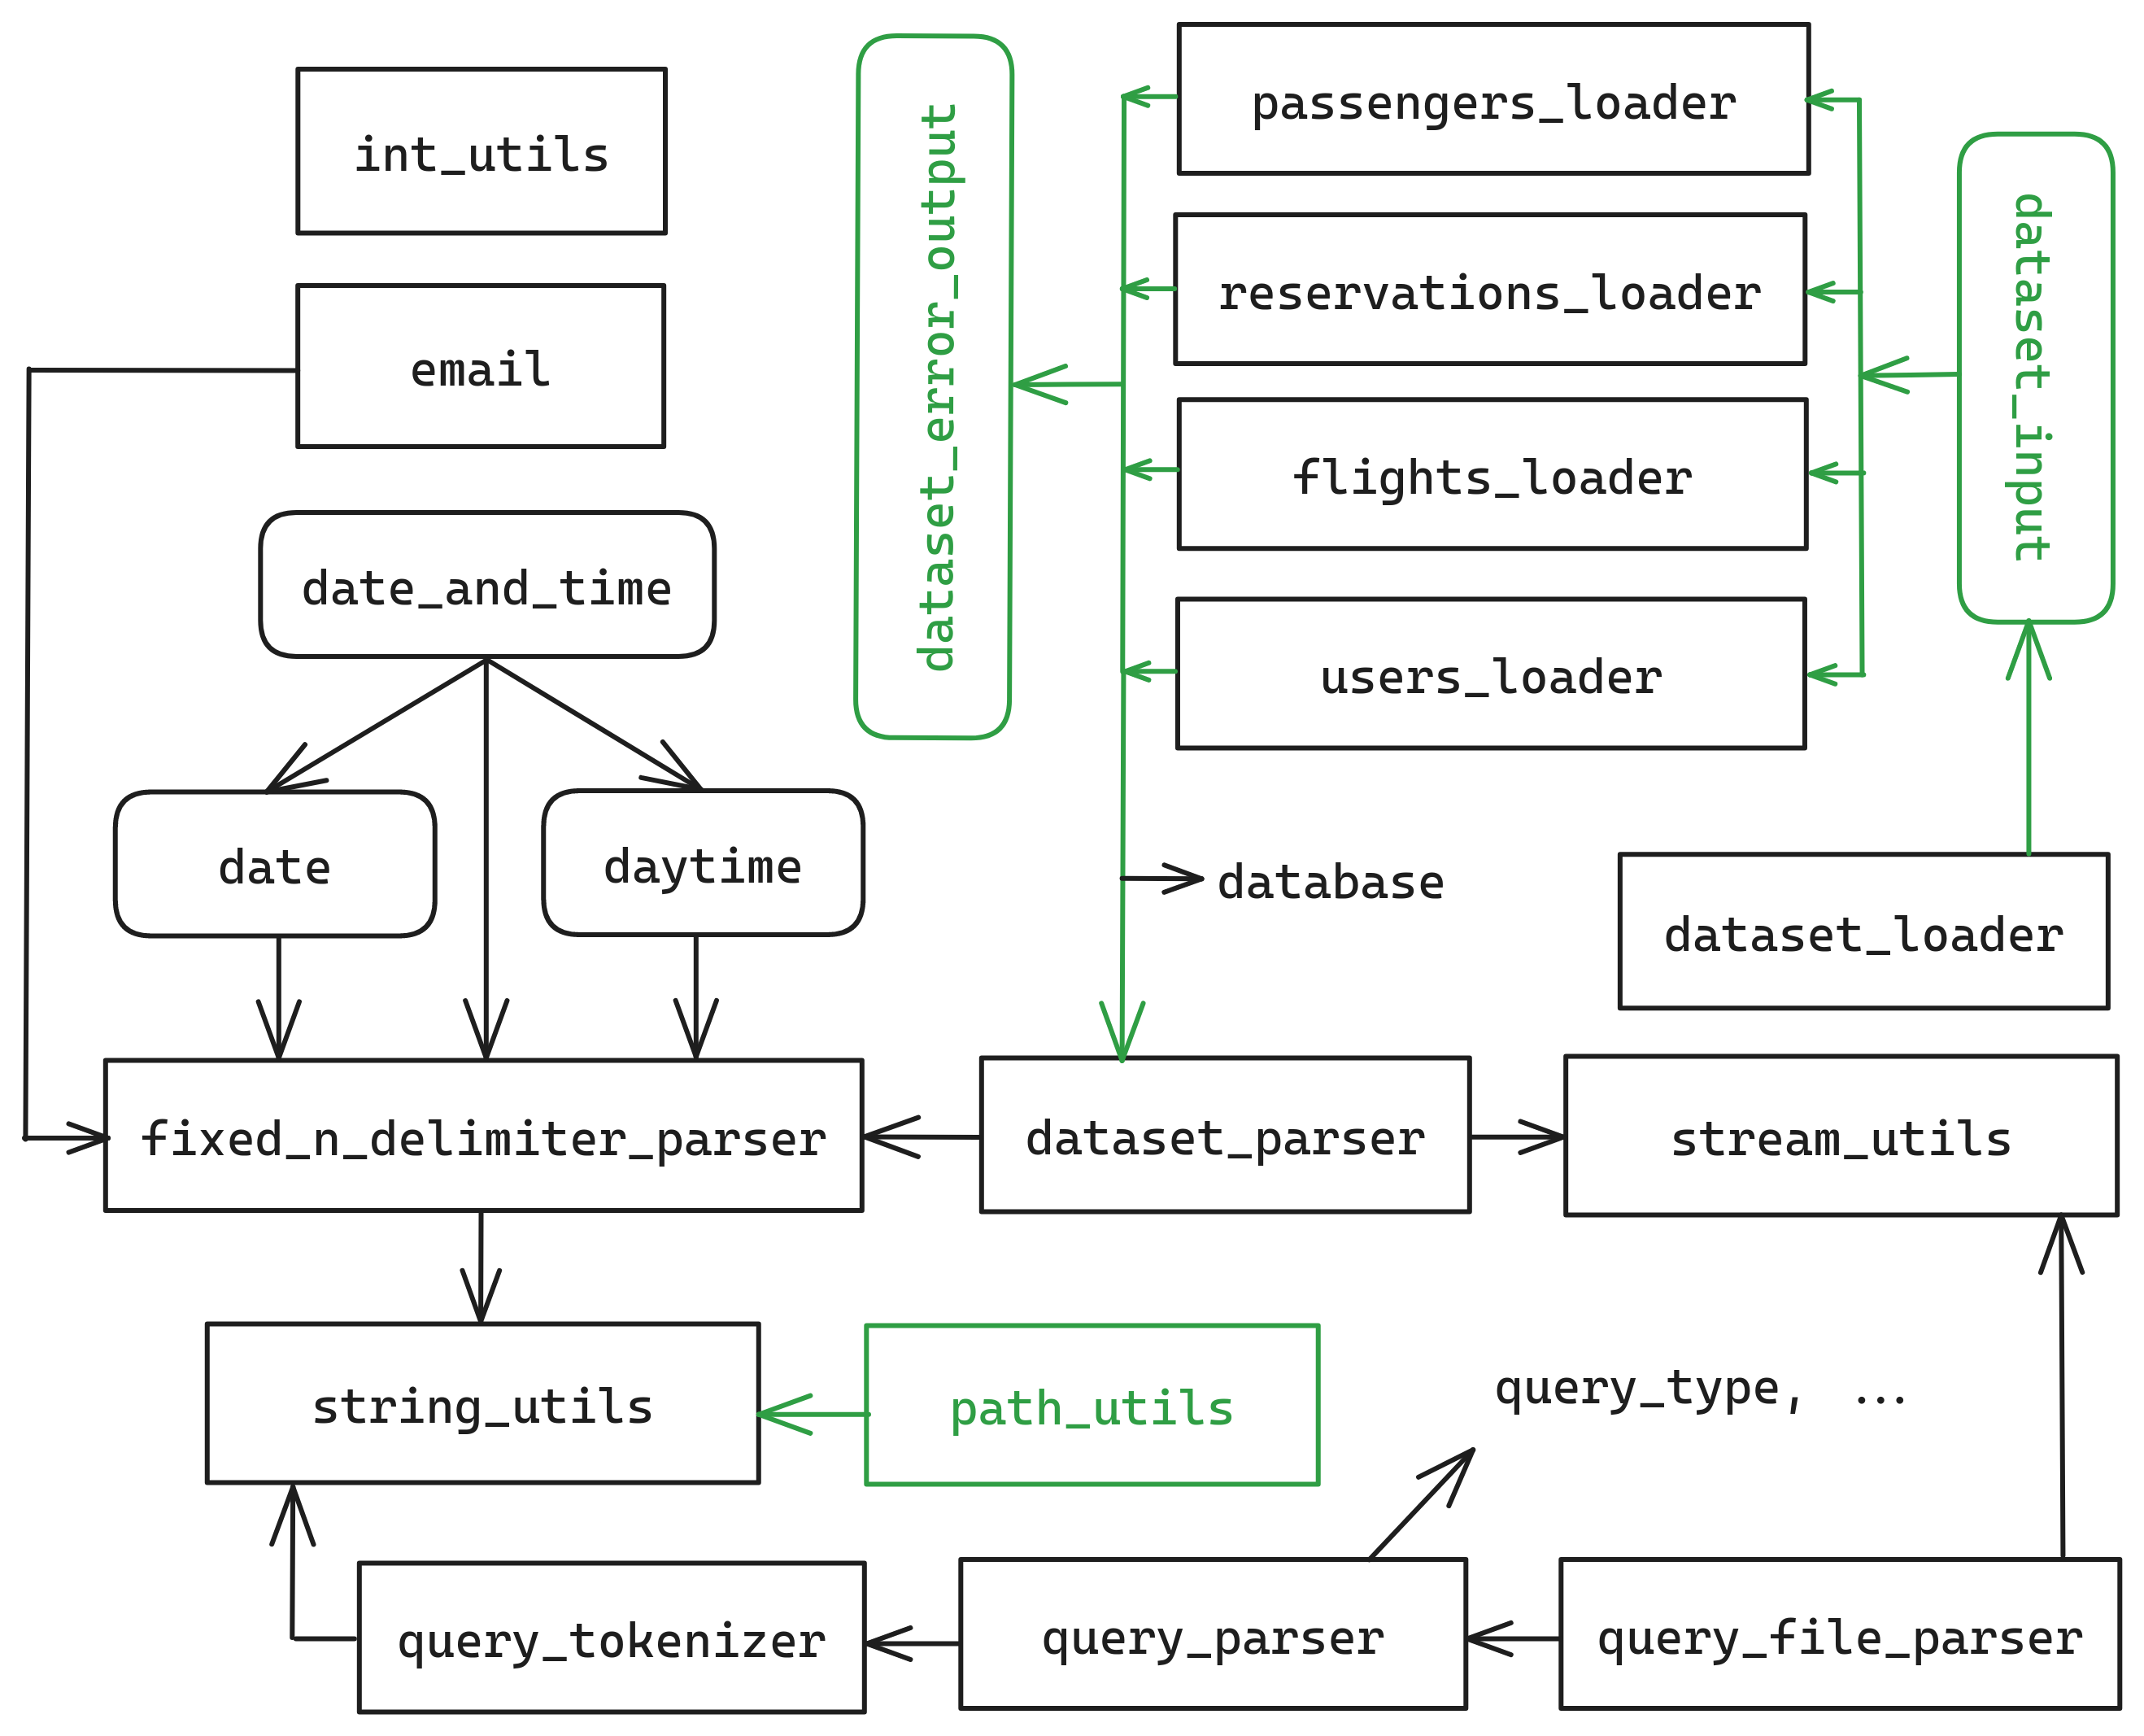
\includegraphics[scale=0.17]{res-fase2/parsing.png}
    \caption{Diagrama de dependências do subsistema de \emph{parsing}}
    \label{fig:parsing}
\end{figure}

Nesta fase do projeto, separámos as funcionalidades de \emph{input} de dados e \emph{output} de
erros num \emph{dataset}, antes concentradas no módulo \texttt{dataset\_loader}. Agora, este módulo
gere duas estruturas de dados distintas, \texttt{dataset\_input} e \texttt{dataset\_error\_output},
formadas por \emph{handles} de ficheiros abertos para leitura / escrita. Ademais, adicionámos o
módulo \texttt{path\_utils}, para manipulação de caminhos para ficheiros.

\subsection{Entidades}
\label{sec:entities}

\begin{figure}[ht]
    \centering
    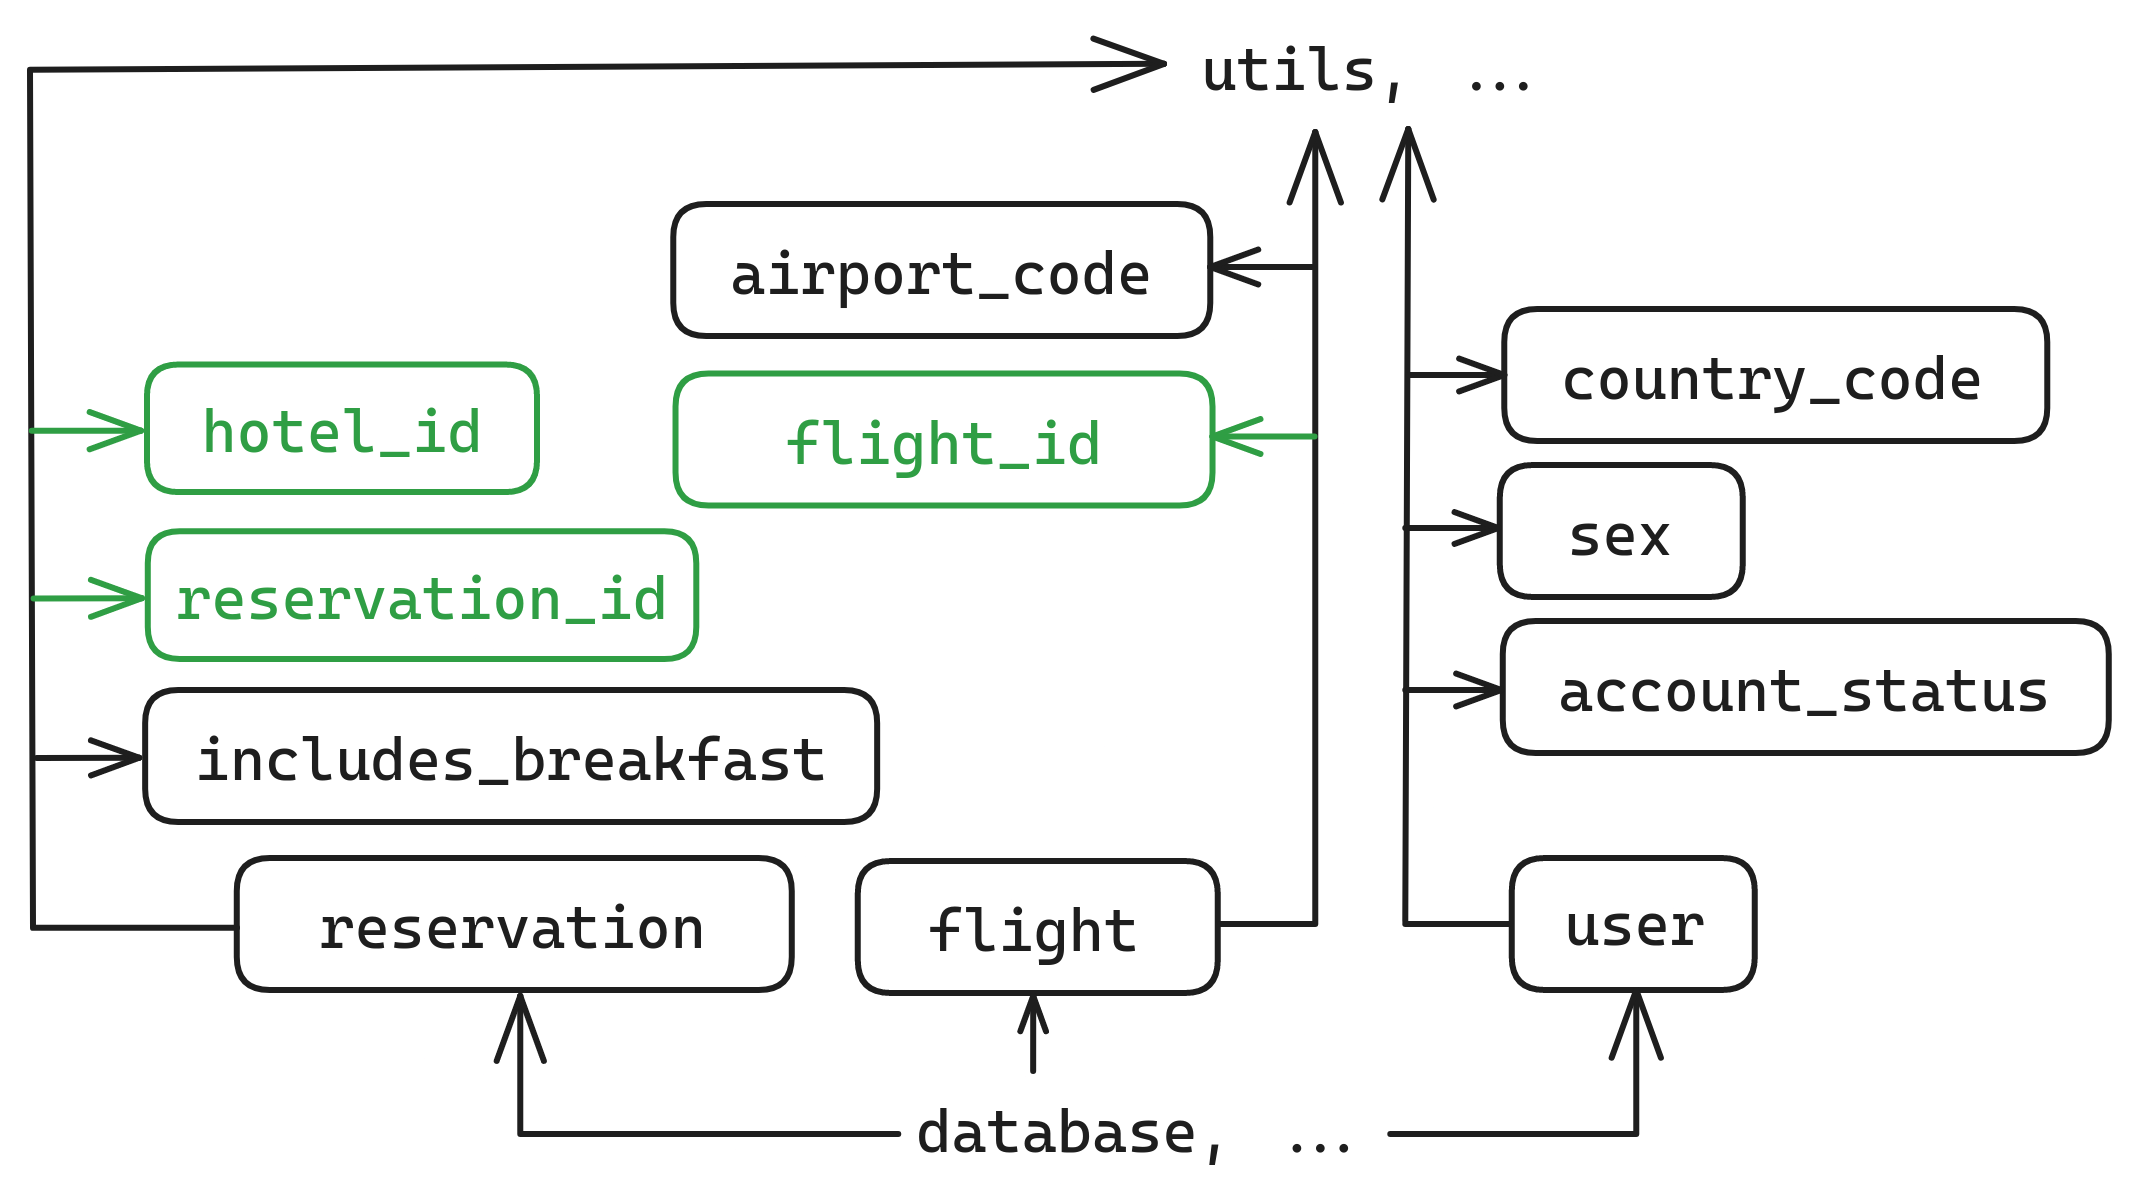
\includegraphics[scale=0.2]{res-fase2/entities.png}
    \caption{Diagrama de dependências das entidades da aplicação}
    \label{fig:entities}
\end{figure}

Nas entidades, criámos módulos para os identificadores de voos, reservas e hotéis. Estes são
armazenados como inteiros, e consequentemente exigem \emph{parsing} e uma forma de serem
apresentados textualmente, código que antes se encontrava em duplicado em vários locais da
aplicação.

\subsection{Catálogos}
\label{sec:catalogs}

\begin{figure}[ht]
    \centering
    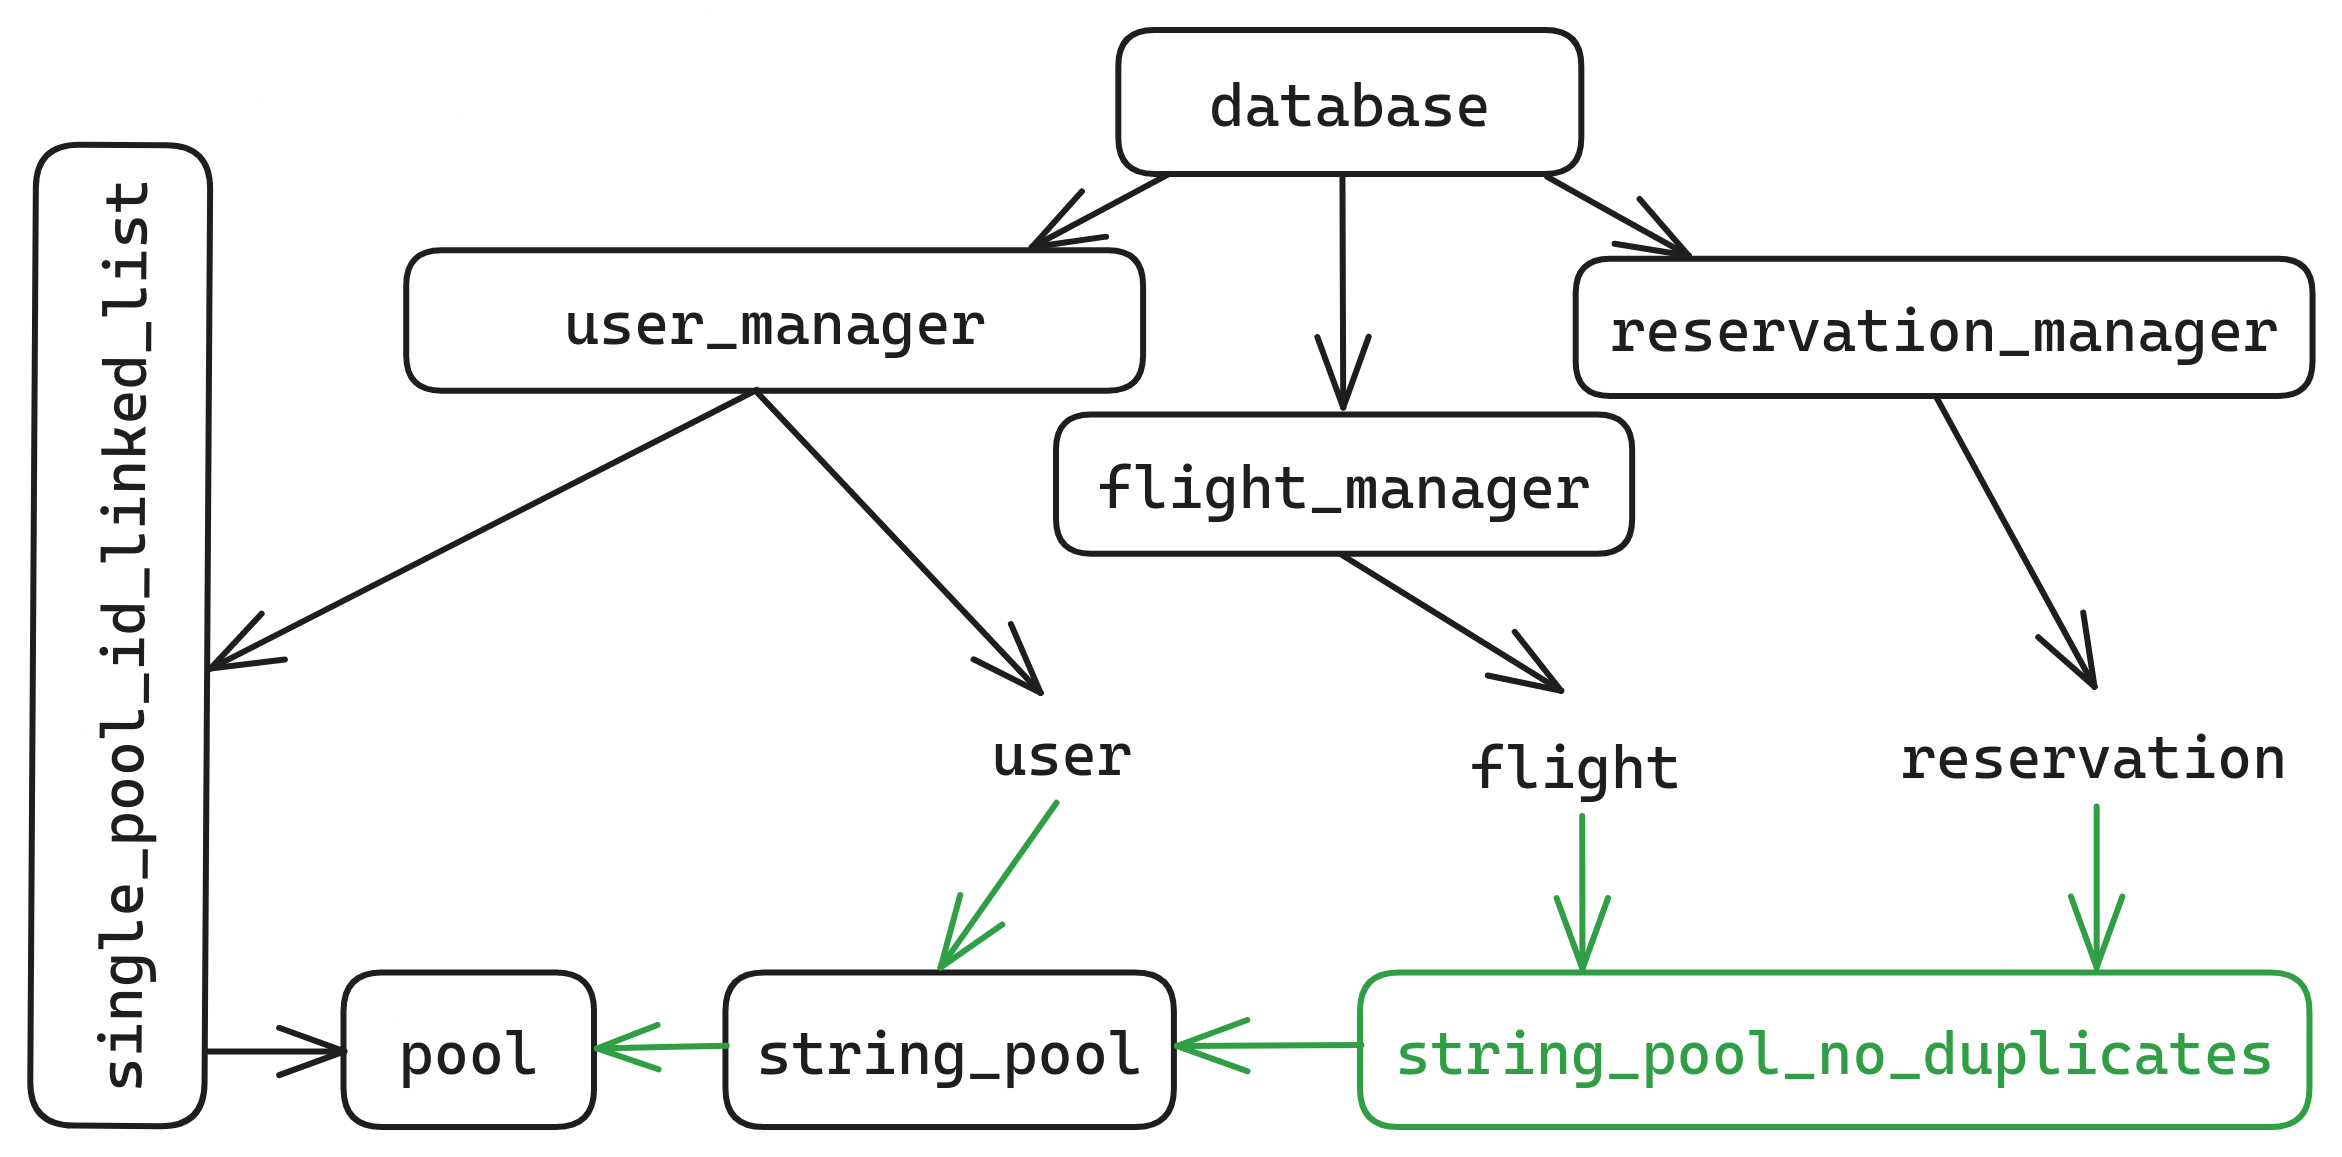
\includegraphics[scale=0.17]{res-fase2/database.png}
    \caption{Diagrama de dependências dos catálogos na aplicação}
    \label{fig:catalogs}
\end{figure}

De modo diminuir o uso de memória da aplicação ainda mais, procurámos comprimir campos do
\emph{dataset} com baixa entropia, como nomes de hotéis e de companhias aérias, que surgem várias
vezes repetidos. Para isso, criámos um novo alocador que armazena \emph{strings} repetidas apenas
uma vez, o \texttt{string\_pool\_no\_duplicates}.

Quanto às novas relações de dependência, reimplementámos a \texttt{string\_pool} utilizando uma
\texttt{pool}, para melhor reutilização de código. Ademais, agora as entidades passam a depender
dos alocadores, por motivos explicados em \nameref{sec:modularity-and-encapsulation}.

\subsection{\emph{Queries}}
\label{sec:queries}

\begin{figure}[ht]
    \centering
    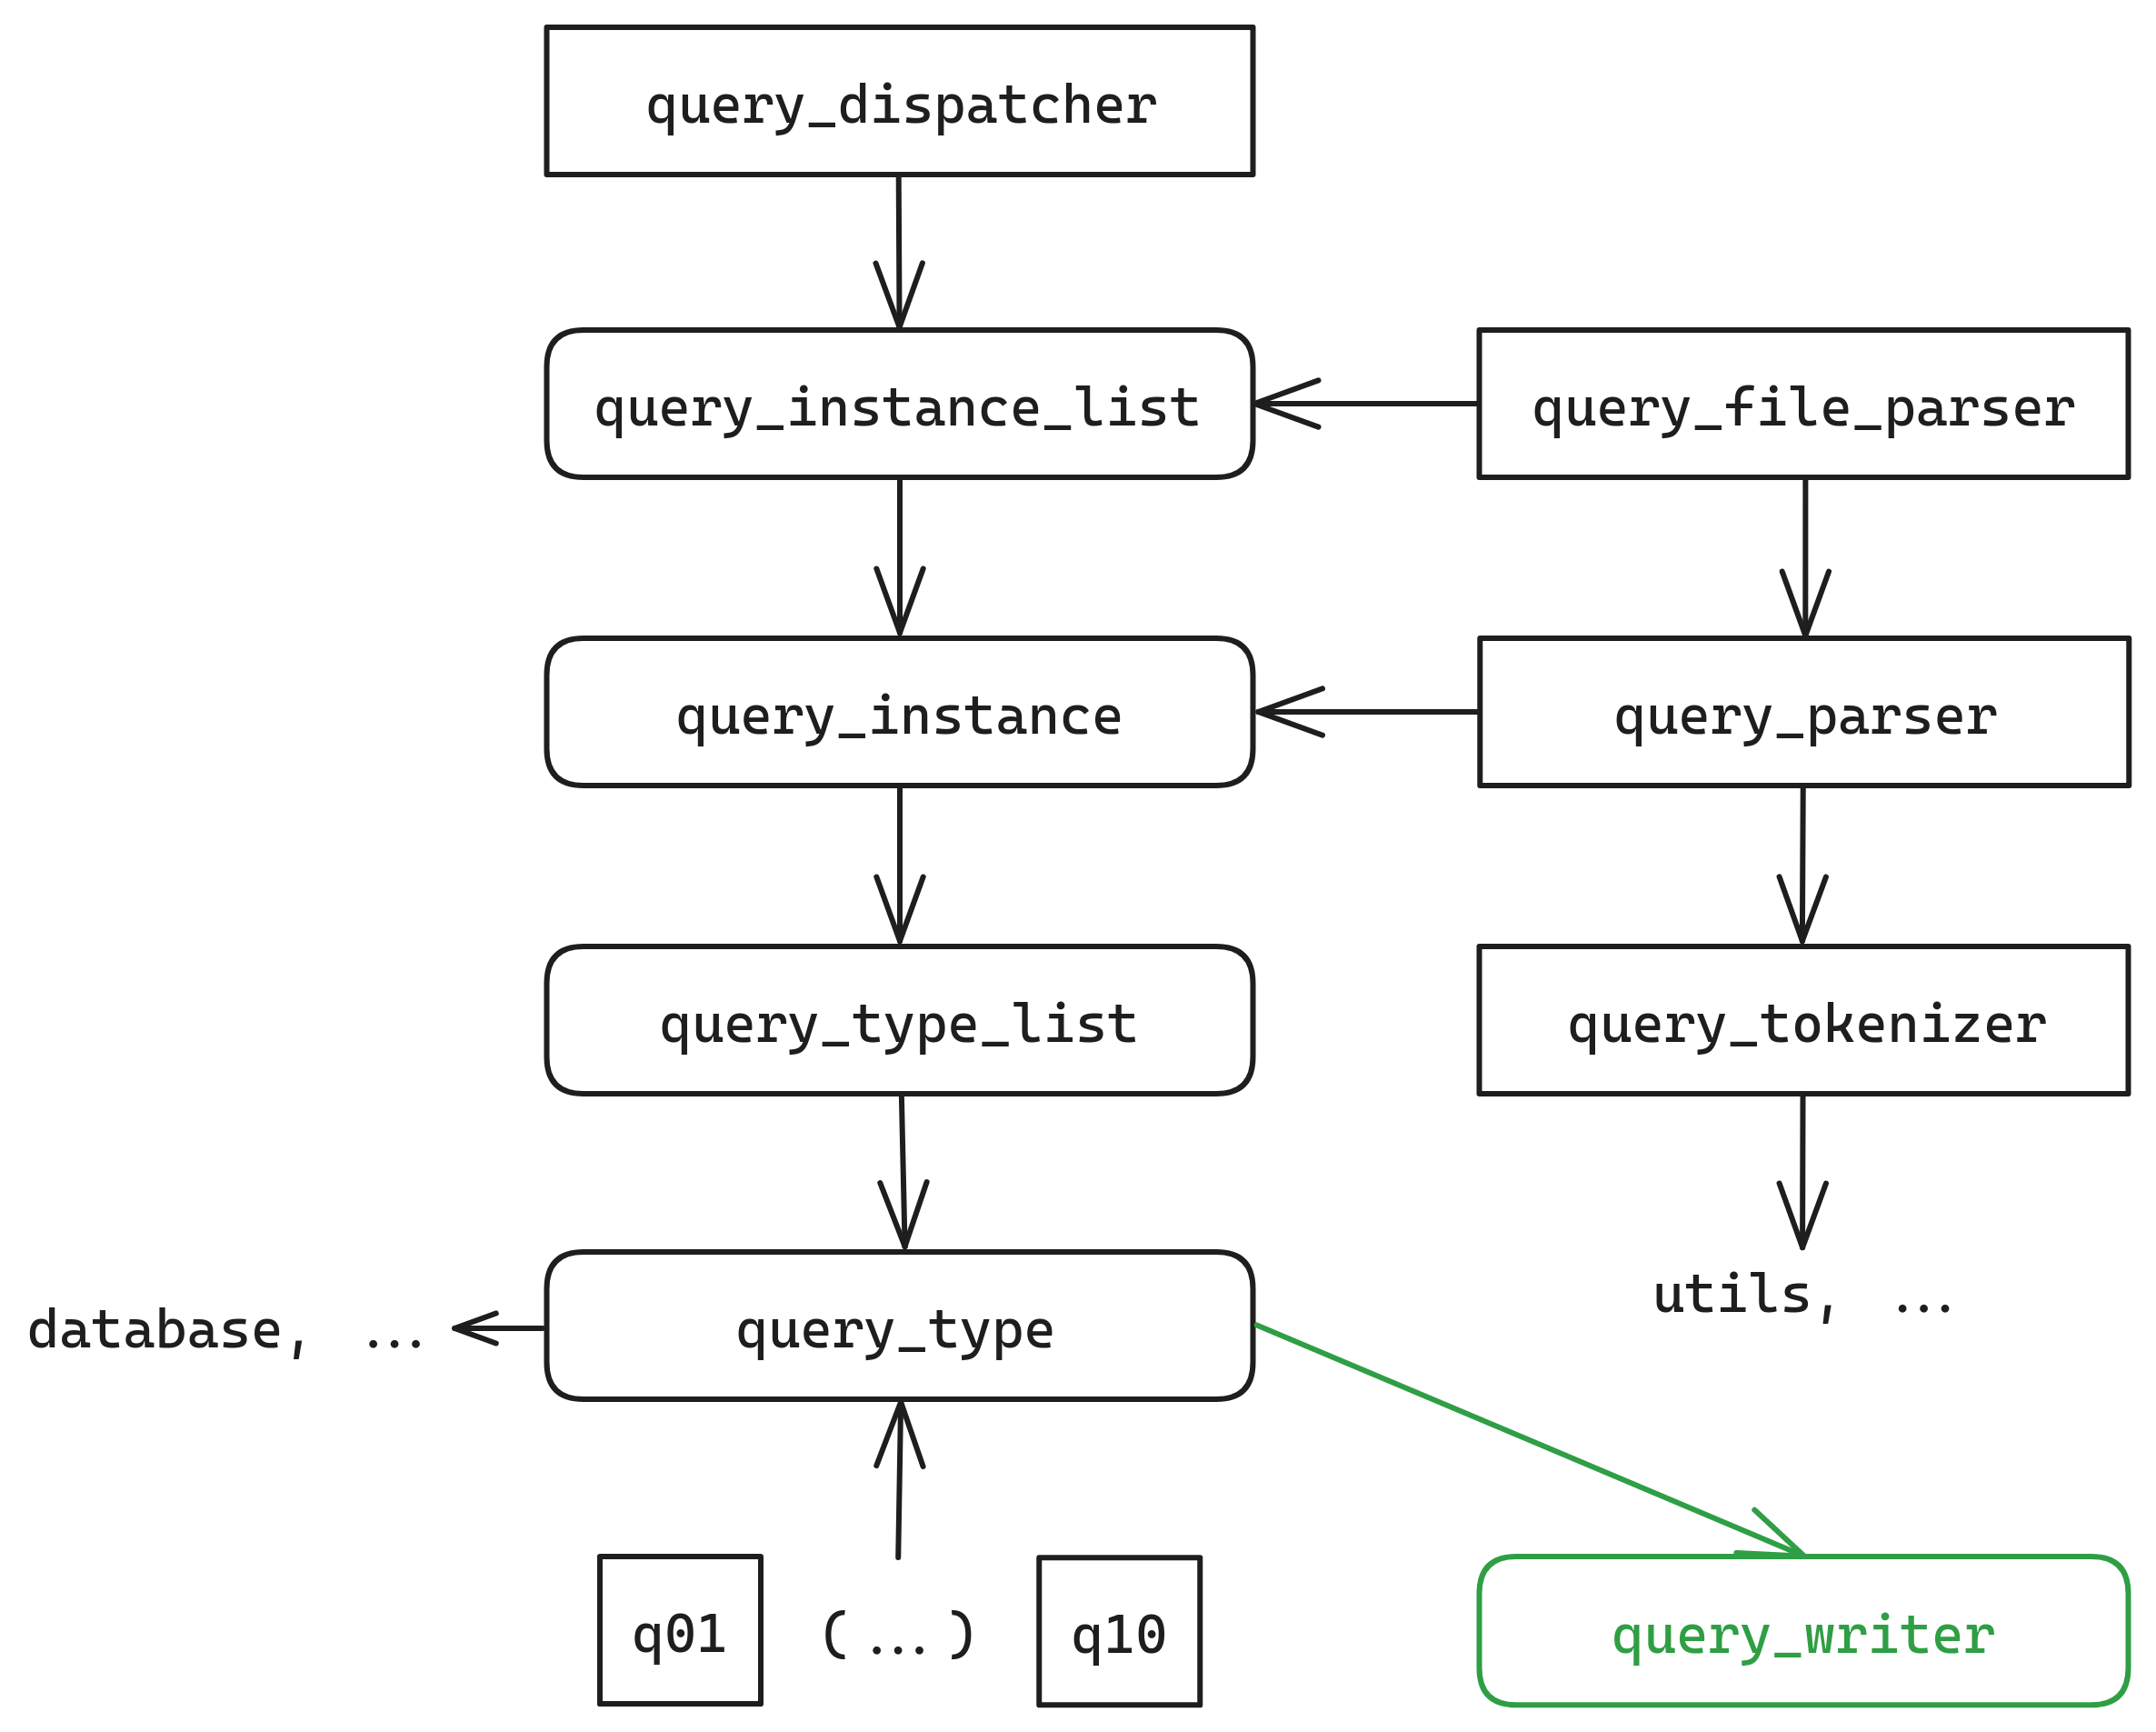
\includegraphics[scale=0.17]{res-fase2/queries.png}
	\caption{Diagrama de dependências do subsistema de \emph{queries}}
    \label{fig:queries}
\end{figure}

Como todas as \emph{queries} apresentam a mesma formatação de \emph{output}, adicionámos a estrutura
\texttt{query\_writer}, que formata o \emph{output} de uma \emph{query} automaticamente, e escreve-o
para um ficheiro (modo \emph{batch}) ou para um conjunto de linhas em memória (modo interativo).
Segue-se a descrição do funcionamento das \emph{queries} novas e das que sofreram mudanças
significativas:

\begin{itemize}
    \item \textbf{Q05} - Listagem dos voos com origem num dado aeroporto entre duas datas. Com uma
                         única iteração pelos voos para todas as \emph{queries} deste tipo,
                         verifica-se se cada voo cumpre as condições para ser parte da resposta
                         de uma \emph{query}. Em caso afirmativo, adiciona-se esse voo a um
                         \emph{array}, associado à \emph{query} através de uma tabela de
                         \emph{hash}. Após cada \emph{array} ser ordenado, a execução de cada
                         \emph{query} consiste simplesmente na exibição dos seus conteúdos.

    \item \textbf{Q07} - Listagem dos aeroportos com maior mediana de atrasos. Inicia-se com uma
                         tabela de \emph{hash} que associa aeroportos a \emph{arrays} de números
                         correspondentes a atrasos. Com uma única iteração pelos voos para todas
                         as \emph{queries} deste tipo, preenche-se o \emph{array} de cada aeroporto
                         com os atrasos dos seus voos. No fim, ordena-se cada \emph{array} e gera-se
                         uma tabela de \emph{hash} entre aeroportos e atrasos. A execução de uma
                         \emph{query} individual consiste na consulta dos maiores elementos desta
                         tabela.

    \item \textbf{Q08} - Cálculo da receita de um hotel entre duas datas. Com uma única iteração
                         pelas reservas para todas as \emph{queries} deste tipo, gera-se uma tabela
                         de \emph{hash} que associa pares hotéis + datas às suas receitas. A cada
                         reserva, calcula-se o número de noites simultaneamente dormidas e no
                         intervalo da \emph{query}, para se calcular a receita resultante dessa
                         reserva. A execução de cada \emph{query} consiste simplesmente na consulta
                         da tabela gerada.

    \item \textbf{Q09} - Listagem de todos os utilizadores cujo nome comece com um dado prefixo. A
                         nova implementação desta \emph{query} é muito semelhante à da \textbf{Q5},
                         mas com uma iteração pelos utilizadores em vez dos voos. Esta solução é
                         significativamente mais veloz que a anterior, que iterava pelos
                         utilizadores uma vez para cada \emph{query}. Considerámos a possibilidade
                         de geração da um índice usando \emph{tries}, mas o seu elevado uso de
                         memória não é compensador, dado que muito pouco do tempo total do programa
                         é passado na execução desta \emph{query}.

    \item \textbf{Q10} - {\color{red}Ainda tenho de implementar isto}
\end{itemize}

\subsection{Modo interativo}
\label{sec:interactive-mode}

\begin{figure}[ht]
    \centering
    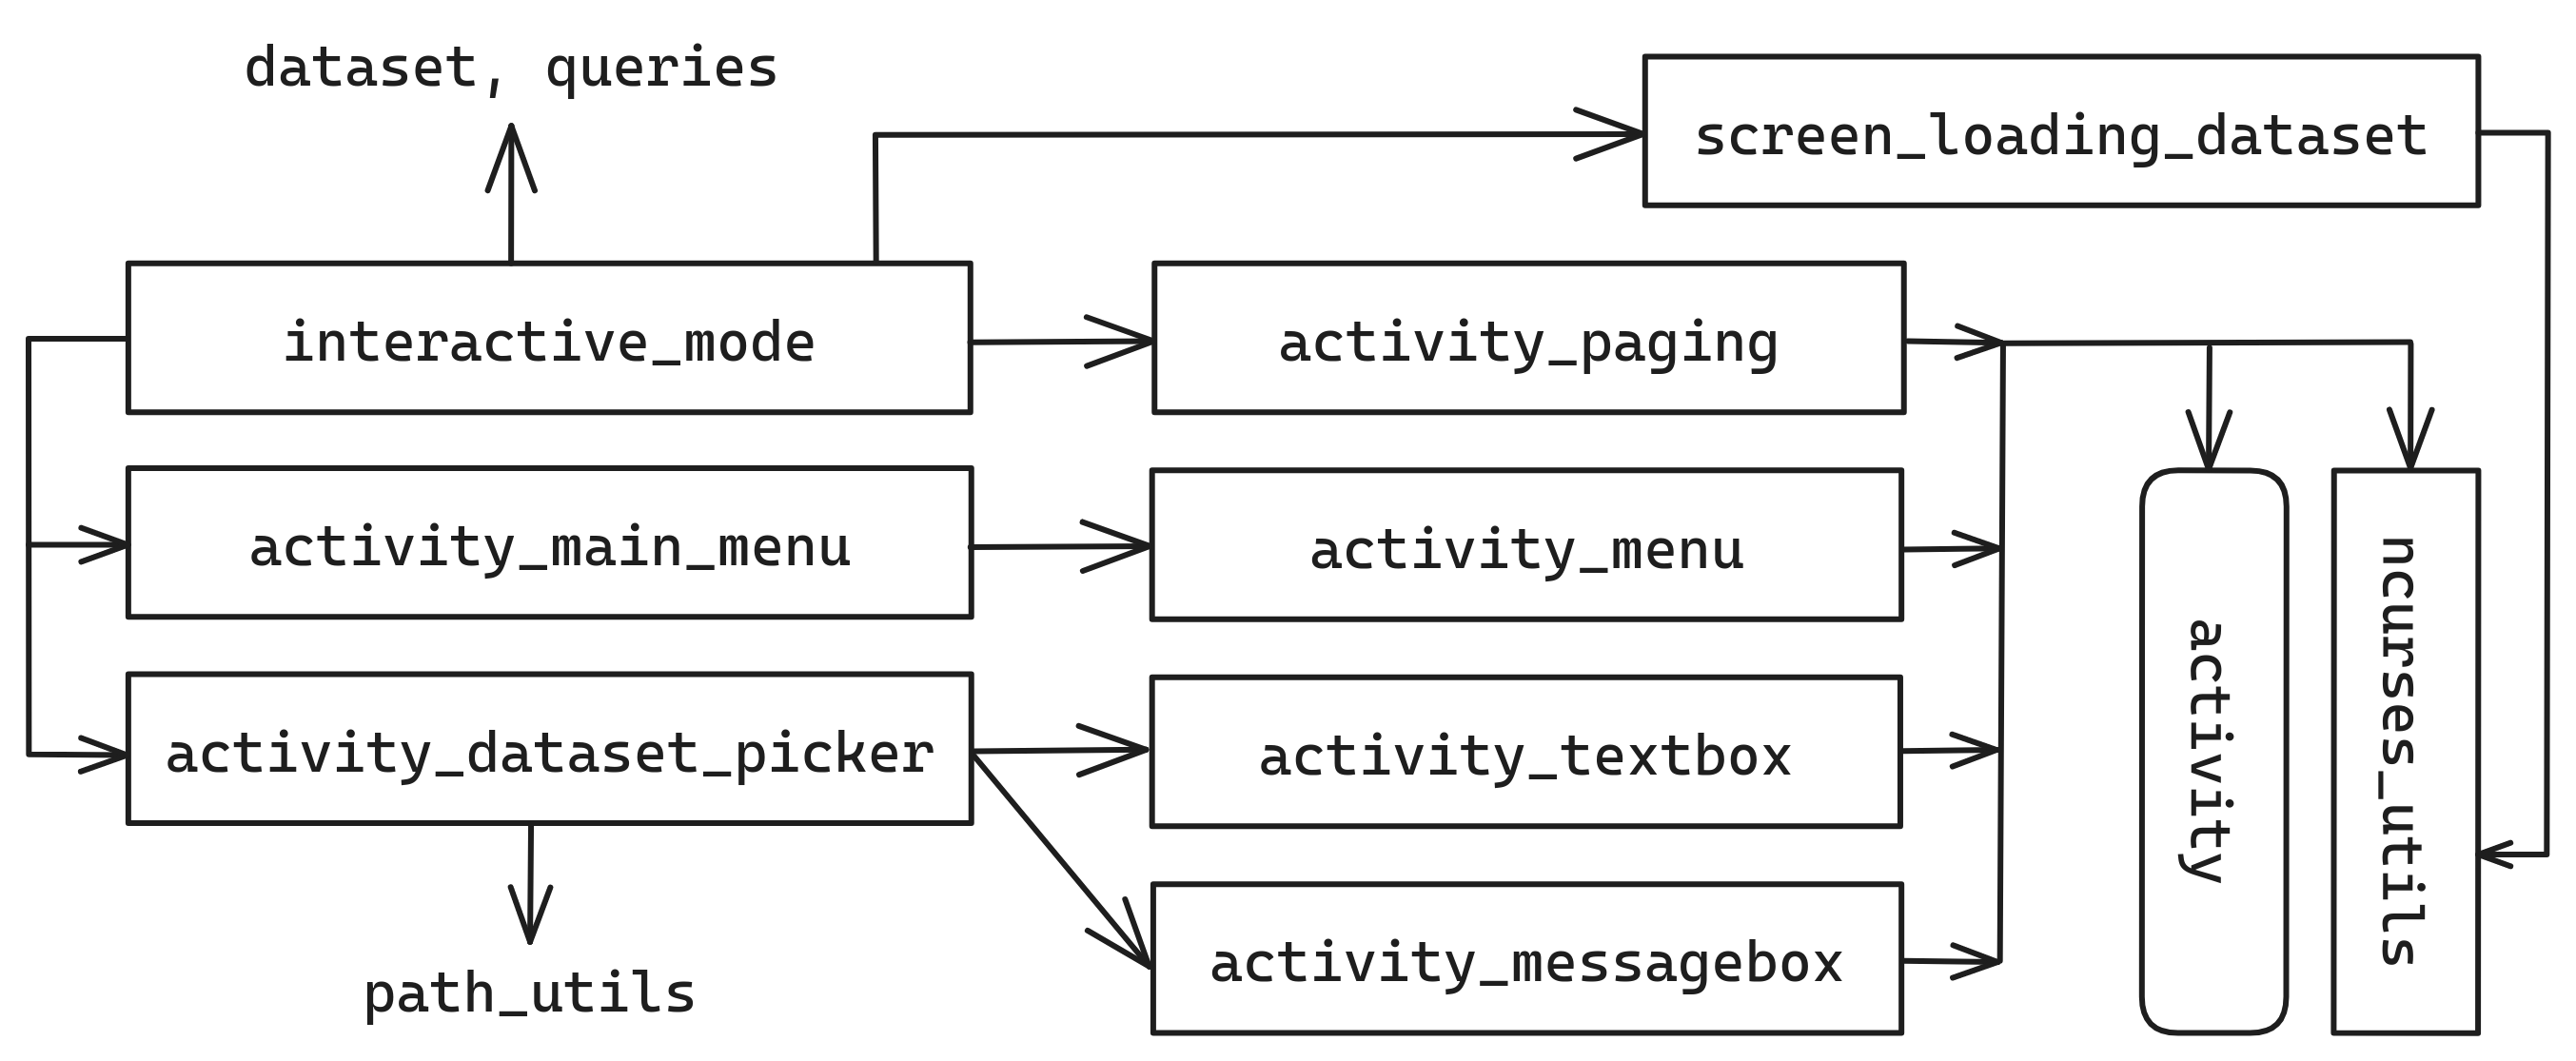
\includegraphics[scale=0.17]{res-fase2/interactive.png}
    \caption{Diagrama de dependências do modo interativo}
    \label{fig:interactive}
\end{figure}

O modo interativo revolve à volta do conceito de atividade (\texttt{activity}), que gere o
\emph{loop} de eventos de uma interface \texttt{curses}, chamando os \emph{callbacks} com os quais
é definida para responder a esses eventos. Imagens de cada uma destas atividades podem ser
encontradas em \nameref{sec:interactive-screenshots}. \texttt{screen\_loading\_dataset} não responde
a eventos, mas desenha no ecrã que a aplicação se encontra a ler um \emph{dataset}. O módulo
\texttt{interactive\_mode} é responsável por controlar a troca entre atividades, formando a
aplicação final.

Fizemos questão de que o modo interativo fosse fácil de utilizar: incluímos instruções em todas as
interfaces, e desenvolvemos um navegador de ficheiros para o utilizador não ter de digitar um
caminho de ficheiro. Ademais, temos excelente suporte para Unicode, com medição textual correta para
o \emph{layout} das interfaces (alguns caracteres podem ser mais longos que outros, situação
com a qual o nosso programa lida corretamente).

\section{Modularidade e encapsulamento}
\label{sec:modularity-and-encapsulation}

\section{Anexos}
\label{sec:annexes}

\subsection{Diagrama de dependências completo}
\label{sec:complete-diagram}

% TODO - full dependency diagram

\subsection{\emph{Screenshots} do modo interativo}
\label{sec:interactive-screenshots}

\end{document}
